\documentclass[tikz,border=6pt]{standalone}
\usepackage[scaled=0.92]{helvet}
\renewcommand{\familydefault}{\sfdefault}
\usepackage{sfmath,amssymb}
\usetikzlibrary{arrows.meta,positioning,calc,fit,backgrounds}
\definecolor{ink}{HTML}{1F2933}\definecolor{mute}{HTML}{5B6670}
\definecolor{usF}{HTML}{ECE6F8}\definecolor{usD}{HTML}{5E3EA8}
\definecolor{enF}{HTML}{DFF3EF}\definecolor{enD}{HTML}{17766A}
\definecolor{agF}{HTML}{E3ECFA}\definecolor{agD}{HTML}{2B5BAA}
\definecolor{cpF}{HTML}{FCF1D8}\definecolor{cpD}{HTML}{A8670A}
\definecolor{grF}{HTML}{C9EBE4}
\definecolor{done}{HTML}{3D7A34}\definecolor{prog}{HTML}{C98A0B}\definecolor{todo}{HTML}{8A949C}
\definecolor{llm}{HTML}{A23B32}\definecolor{llmF}{HTML}{F9E0DE}
\tikzset{
 panel/.style={draw=#1,line width=0.9pt,rounded corners=5pt},
 hd/.style={font=\bfseries\large,text=ink,anchor=north west},
 sub/.style={font=\small,text=mute,anchor=north west},
 bx/.style={draw=#1,fill=white,rounded corners=3pt,line width=0.7pt,align=center,font=\small,text=ink,inner sep=4pt},
 tk/.style={draw=enD,fill=grF,rounded corners=3pt,line width=0.8pt,align=center,font=\small\bfseries,text=ink,minimum height=0.95cm,inner sep=3pt},
 ar/.style={-{Stealth[length=6pt,width=5pt]},line width=1pt,color=ink!75},
 ms/.style={rounded corners=3pt,line width=0.8pt,align=left,font=\footnotesize,text=ink,inner sep=3pt,anchor=north west,text width=#1},
}
\begin{document}
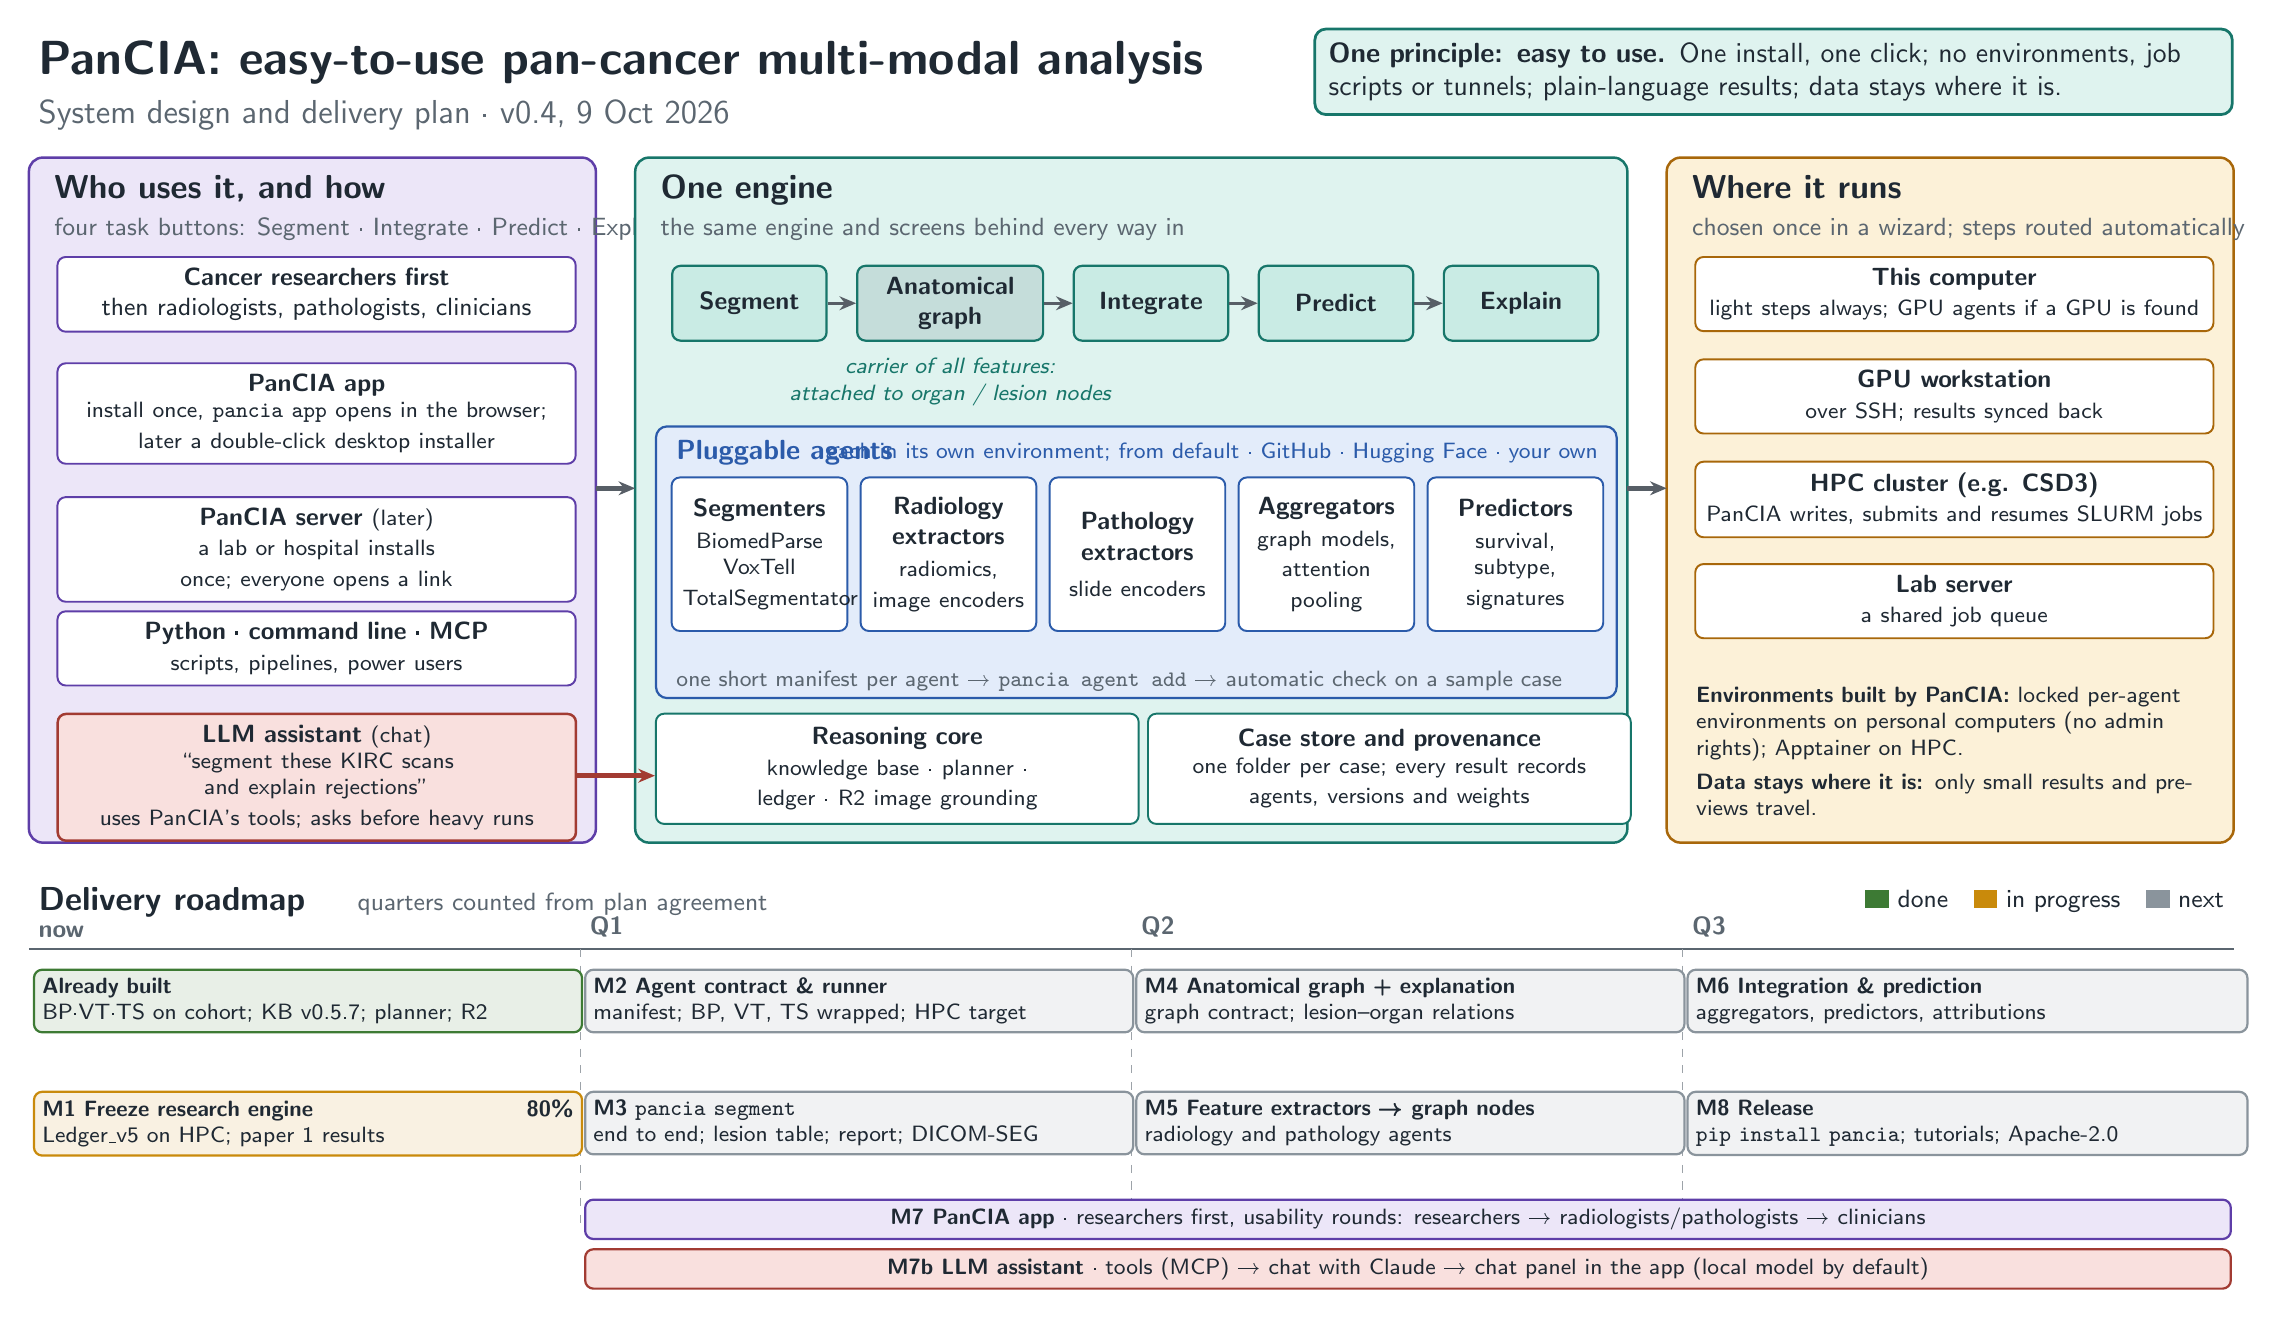
\begin{tikzpicture}[x=1cm,y=1cm]
% ===== title + principle
\node[anchor=north west,font=\bfseries\LARGE,text=ink] at (0,15.2) {PanCIA: easy-to-use pan-cancer multi-modal analysis};
\node[anchor=north west,font=\large,text=mute] at (0,14.45) {System design and delivery plan \textperiodcentered\ v0.4, 9 Oct 2026};
\node[anchor=north east,draw=enD,fill=enF,rounded corners=4pt,line width=1pt,align=left,font=\normalsize,text=ink,inner sep=5pt,text width=11.3cm] at (28,15.25)
 {\textbf{One principle: easy to use.} One install, one click; no environments, job scripts or tunnels; plain-language results; data stays where it is.};

% ===== panel A: people and front doors
\draw[panel=usD,fill=usF] (0,4.9) rectangle (7.2,13.6);
\node[hd] at (0.2,13.5) {Who uses it, and how};
\node[sub] at (0.2,12.95) {four task buttons: Segment \textperiodcentered\ Integrate \textperiodcentered\ Predict \textperiodcentered\ Explain};
\node[bx=usD,text width=6.3cm,anchor=north west] (u) at (0.35,12.35)
 {\textbf{Cancer researchers first}\\ then radiologists, pathologists, clinicians};
\node[bx=usD,text width=6.3cm,anchor=north west] (d1) at (0.35,11.0)
 {\textbf{PanCIA app}\\ \footnotesize install once, \texttt{pancia app} opens in the browser;\\ \footnotesize later a double-click desktop installer};
\node[bx=usD,text width=6.3cm,anchor=north west] (d2) at (0.35,9.3)
 {\textbf{PanCIA server} {\footnotesize(later)}\\ \footnotesize a lab or hospital installs once; everyone opens a link};
\node[bx=usD,text width=6.3cm,anchor=north west] (d3) at (0.35,7.85)
 {\textbf{Python \textperiodcentered\ command line \textperiodcentered\ MCP}\\ \footnotesize scripts, pipelines, power users};
\node[draw=llm,fill=llmF,rounded corners=3pt,line width=0.9pt,align=center,font=\small,text=ink,text width=6.3cm,anchor=north west,inner sep=4pt] (llm) at (0.35,6.55)
 {\textbf{LLM assistant} {\footnotesize(chat)}\\ \footnotesize``segment these KIRC scans and explain rejections''\\ \footnotesize uses PanCIA's tools; asks before heavy runs};

% ===== panel B: engine
\draw[panel=enD,fill=enF] (7.7,4.9) rectangle (20.3,13.6);
\node[hd] at (7.9,13.5) {One engine};
\node[sub] at (7.9,12.95) {the same engine and screens behind every way in};
\node[tk,text width=1.75cm] (t1) at (9.15,11.75) {Segment};
\node[tk,text width=2.15cm,fill=enD!25] (t2) at (11.7,11.75) {Anatomical\\graph};
\node[tk,text width=1.75cm] (t3) at (14.25,11.75) {Integrate};
\node[tk,text width=1.75cm] (t4) at (16.6,11.75) {Predict};
\node[tk,text width=1.75cm] (t5) at (18.95,11.75) {Explain};
\foreach \a/\b in {t1/t2,t2/t3,t3/t4,t4/t5} \draw[ar] (\a) -- (\b);
\node[font=\footnotesize\itshape,text=enD,align=center] at (11.7,10.75) {carrier of all features:\\ attached to organ / lesion nodes};
% agents
\node[draw=agD,fill=agF,rounded corners=4pt,line width=0.8pt,minimum width=12.2cm,minimum height=3.45cm,anchor=north west] (ag) at (7.95,10.2) {};
\node[anchor=north west,font=\bfseries\normalsize,text=agD] at (8.1,10.13) {Pluggable agents};
\node[anchor=north east,font=\footnotesize,text=agD] at (20.05,10.1) {each in its own environment; from default \textperiodcentered\ GitHub \textperiodcentered\ Hugging Face \textperiodcentered\ your own};
\node[bx=agD,anchor=north west,text width=1.95cm,minimum height=1.95cm] at (8.15,9.55) {\textbf{Segmenters}\\[2pt]\footnotesize BiomedParse\\VoxTell\\TotalSegmentator};
\node[bx=agD,anchor=north west,text width=1.95cm,minimum height=1.95cm] at (10.55,9.55) {\textbf{Radiology\\extractors}\\[2pt]\footnotesize radiomics,\\image encoders};
\node[bx=agD,anchor=north west,text width=1.95cm,minimum height=1.95cm] at (12.95,9.55) {\textbf{Pathology\\extractors}\\[2pt]\footnotesize slide encoders};
\node[bx=agD,anchor=north west,text width=1.95cm,minimum height=1.95cm] at (15.35,9.55) {\textbf{Aggregators}\\[2pt]\footnotesize graph models,\\attention pooling};
\node[bx=agD,anchor=north west,text width=1.95cm,minimum height=1.95cm] at (17.75,9.55) {\textbf{Predictors}\\[2pt]\footnotesize survival, subtype,\\signatures};
\node[anchor=north west,font=\footnotesize,text=mute] at (8.1,7.2) {one short manifest per agent \textrightarrow\ \texttt{pancia agent add} \textrightarrow\ automatic check on a sample case};
% core
\node[bx=enD,anchor=north west,text width=5.85cm,minimum height=1.4cm] at (7.95,6.55)
 {\textbf{Reasoning core}\\ \footnotesize knowledge base \textperiodcentered\ planner \textperiodcentered\ ledger \textperiodcentered\ R2 image grounding};
\node[bx=enD,anchor=north west,text width=5.85cm,minimum height=1.4cm] at (14.2,6.55)
 {\textbf{Case store and provenance}\\ \footnotesize one folder per case; every result records\\ \footnotesize agents, versions and weights};

% ===== panel C: compute
\draw[panel=cpD,fill=cpF] (20.8,4.9) rectangle (28,13.6);
\node[hd] at (21.0,13.5) {Where it runs};
\node[sub] at (21.0,12.95) {chosen once in a wizard; steps routed automatically};
\node[bx=cpD,anchor=north west,text width=6.3cm] at (21.15,12.35) {\textbf{This computer}\\ \footnotesize light steps always; GPU agents if a GPU is found};
\node[bx=cpD,anchor=north west,text width=6.3cm] at (21.15,11.05) {\textbf{GPU workstation}\\ \footnotesize over SSH; results synced back};
\node[bx=cpD,anchor=north west,text width=6.3cm] at (21.15,9.75) {\textbf{HPC cluster (e.g. CSD3)}\\ \footnotesize PanCIA writes, submits and resumes SLURM jobs};
\node[bx=cpD,anchor=north west,text width=6.3cm] at (21.15,8.45) {\textbf{Lab server}\\ \footnotesize a shared job queue};
\node[anchor=north west,align=left,font=\footnotesize,text=ink,text width=6.5cm] at (21.05,7.0)
 {\textbf{Environments built by PanCIA:} locked per-agent environments on personal computers (no admin rights); Apptainer on HPC.\\[3pt]
  \textbf{Data stays where it is:} only small results and previews travel.};

% arrows between panels
\draw[ar,line width=1.6pt] (7.2,9.4) -- (7.7,9.4);
\draw[ar,line width=1.6pt] (20.3,9.4) -- (20.8,9.4);
\draw[ar,line width=1.6pt,color=llm] (6.95,5.75) -- (7.95,5.75);

% ===== roadmap
\node[anchor=north west,font=\bfseries\large,text=ink] at (0,4.45) {Delivery roadmap};
\node[anchor=north west,font=\small,text=mute] at (4.05,4.38) {quarters counted from plan agreement};

\node[anchor=north east,font=\small,text=ink] at (28,4.42) {\tikz\fill[done](0,0)rectangle(0.3,0.22); done\quad \tikz\fill[prog](0,0)rectangle(0.3,0.22); in progress\quad \tikz\fill[todo](0,0)rectangle(0.3,0.22); next};
% time axis
\draw[mute,line width=0.6pt] (0,3.55) -- (28,3.55);
\foreach \x/\l in {0/now, 7/Q1, 14/Q2, 21/Q3} \node[anchor=south west,font=\small\bfseries,text=mute] at (\x,3.57) {\l};
\foreach \x in {7,14,21} \draw[mute!60,dashed] (\x,3.55) -- (\x,0);
% milestone cards (x, width, row y, colour, title, text)
\newcommand{\ms}[6]{\node[ms=#2cm,draw=#4,fill=#4!12] at (#1,#3) {\textbf{#5}\\ #6};}
\ms{0.05}{6.75}{1.75}{prog}{M1 Freeze research engine \hfill 80\%}{Ledger\_v5 on HPC; paper 1 results}
\ms{0.05}{6.75}{3.3}{done}{Already built}{BP\textperiodcentered VT\textperiodcentered TS on cohort; KB v0.5.7; planner; R2}
\ms{7.05}{6.75}{3.3}{todo}{M2 Agent contract \& runner}{manifest; BP, VT, TS wrapped; HPC target}
\ms{7.05}{6.75}{1.75}{todo}{M3 \texttt{pancia segment}}{end to end; lesion table; report; DICOM-SEG}
\ms{14.05}{6.75}{3.3}{todo}{M4 Anatomical graph + explanation}{graph contract; lesion--organ relations}
\ms{14.05}{6.75}{1.75}{todo}{M5 Feature extractors \textrightarrow\ graph nodes}{radiology and pathology agents}
\ms{21.05}{6.9}{3.3}{todo}{M6 Integration \& prediction}{aggregators, predictors, attributions}
\ms{21.05}{6.9}{1.75}{todo}{M8 Release}{\texttt{pip install pancia}; tutorials; Apache-2.0}
% cross-cutting bars
\node[anchor=north west,draw=usD,fill=usF,rounded corners=3pt,line width=0.8pt,minimum width=20.9cm,minimum height=0.5cm,font=\footnotesize,text=ink,inner sep=2pt] at (7.05,0.38)
 {\textbf{M7 PanCIA app} \textperiodcentered\ researchers first, usability rounds: researchers \textrightarrow\ radiologists/pathologists \textrightarrow\ clinicians};
\node[anchor=north west,draw=llm,fill=llmF,rounded corners=3pt,line width=0.8pt,minimum width=20.9cm,minimum height=0.5cm,font=\footnotesize,text=ink,inner sep=2pt] at (7.05,-0.25)
 {\textbf{M7b LLM assistant} \textperiodcentered\ tools (MCP) \textrightarrow\ chat with Claude \textrightarrow\ chat panel in the app (local model by default)};
\end{tikzpicture}
\end{document}
